\documentclass{beamer}
\usetheme{Madrid}
\usepackage{lmodern}
\usepackage{hyperref}
\usepackage{apacite}
\usepackage[utf8]{inputenc}
\usepackage[spanish]{babel}

\usepackage{xcolor}
\setbeamertemplate{background}{\tikz[overlay,remember picture]\node[opacity=0.2]at (current page.center){
\includegraphics[width=13cm]{KL.png}};}
\usepackage{tikz}
\usepackage{kantlipsum}

\setbeamercolor{normal text}{fg=black}

\begin{document}
\colorlet{beamer@blendedblue}{blue!46!green}
\setbeamercolor{normal text}{fg=black}

\setbeamercolor{frametitle}{fg=white, bg=blue!46!green}
\setbeamercolor*{title}{bg=blue!46!green, fg=white}

\setbeamercolor{section in toc}{fg=black}

\author[Juan C. Correa \textcolor{white}{(\url{https://correajc.com}})]{Juan C. Correa, Ph.D.}
\title[TREME 5: Preprints y Ciencia Abierta]{Preprints y la Ciencia Abierta}
% \subtitle{TREME}
	%\subtitle{}
\institute[]{Fundación Universitaria Konrad Lorenz\\
	\color{blue}\Email  \href{mailto:juanc.correan@konradlorenz.edu.co}{juanc.correan@konradlorenz.edu.co}}
\pgfdeclareimage[height=0.5cm]{KL}{KL}
\logo{\pgfuseimage{KL}}
\setbeamertemplate{caption}[numbered]
\date[Bogotá, Junio-2021]{Curso en: \textbf{T}ecnologías \textbf{R}eproducibles en la \textbf{E}nseñanza de la \textbf{M}etodología y la \textbf{E}stadística}

%\subject{}
\setbeamercolor{background canvas}{bg=white}
%\setbeamertemplate{navigation symbols}{}

\begin{frame}
	\titlepage
\end{frame}

%\setbeamertemplate{background}{\tikz[overlay,remember picture]\node[opacity=0.15]at (current page.center){
\includegraphics[width=14.7cm]{kblack.png}};}


\begin{frame}
\frametitle{Agenda} 
\tableofcontents
\end{frame}

\section{¿Qué es un preprint?}
\begin{frame}{¿Qué es un preprint?}
\Large
Es la versión de un artículo científico que precede a la versión oficialmente publicada por una revista indexada.
\begin{figure}
\centering
 
\includegraphics[width=.2\textwidth]{Wikipedia}
\end{figure}
Frecuentemente está disponible en un formato que no necesariamente coincide con el formato oficial de la revista* 
\end{frame}

\begin{frame}{¿Qué es un preprint?}
\begin{figure}
\centering
 
\includegraphics[width=.9\textwidth]{Tools.png}
\end{figure}
\textcolor{blue}{\url{https://youtu.be/s3JldKoA0zw}}
\end{frame}

\begin{frame}
\Huge
\centering
¿Por qué surgen los preprints?\\
\vspace{1.5cm}
\pause
Veamos un poco de historia
\end{frame}

\section{El Criterio Ingelfinger}
\begin{frame}{El Criterio Ingelfinger}
Franz J. Ingelfinger estableció que \textit{The New England Journal of Medicine} no publicaría hallazgos científicos que ya se encontraran disponibles en cualquier otro formato distinto.
\begin{figure}
\centering
 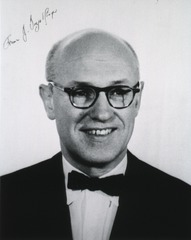
\includegraphics[width=.25\textwidth]{Ingelfinger}
\end{figure}
Este criterio se aplicó con rapidez en otras revistas, porque garantizaba que el contenido publicado era reciente, original (no duplicado) o resultado de plagio.
\end{frame}

\begin{frame}{El Criterio Ingelfinger}
\begin{figure}
\centering
 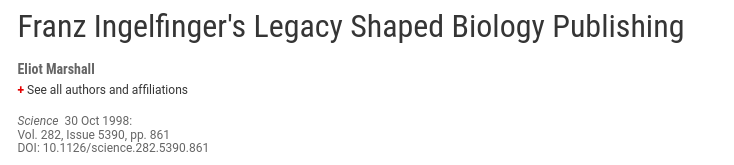
\includegraphics[width=.9\textwidth]{Science}
\end{figure}
\end{frame}

\begin{frame}{El Criterio Ingelfinger}
\begin{figure}
\centering
 
\includegraphics[width=.5\textwidth]{review}
\end{figure}
\end{frame}

\begin{frame}{El Criterio Ingelfinger}
\Large
\centering
¡La revisión por pares es lenta y sujeta a errores!
\end{frame}

\section{Los Primeros Repositorios}
\begin{frame}{Los Primeros Repositorios}
En 1990 Joanne Cohn comenzó a divulgar preprints de física a sus colegas a través de correos electrónicos. Estos correos estaban en formato \TeX{}.
\vspace{0.5cm}
\pause\\
En Agosto 1991, Paul Ginsparg reconoció la necesidad de un servidor central donde guardar todos los preprints y se creó el repositorio LANL.
\vspace{0.5cm}
\pause\\
Rápidamente, los preprints se extendieron a biología cuantitativa y estadística.\vspace{0.5cm}
\pause\\
Finalmente, en 2001 el repositorio LANL se rebautizó como ArXiV que desde entonces es mantenido por la Universidad de Cornell.
\end{frame}

\begin{frame}{Los Primeros Repositorios}
\centering
\begin{figure}
 
\includegraphics[width=.7\textwidth]{arxivyoutube.png}
\end{figure}
\url{https://youtu.be/ntoxZzh0ha8}
\end{frame}


\section{Preprints como solución}
\begin{frame}{Preprints como solución}
\begin{figure}
\centering
 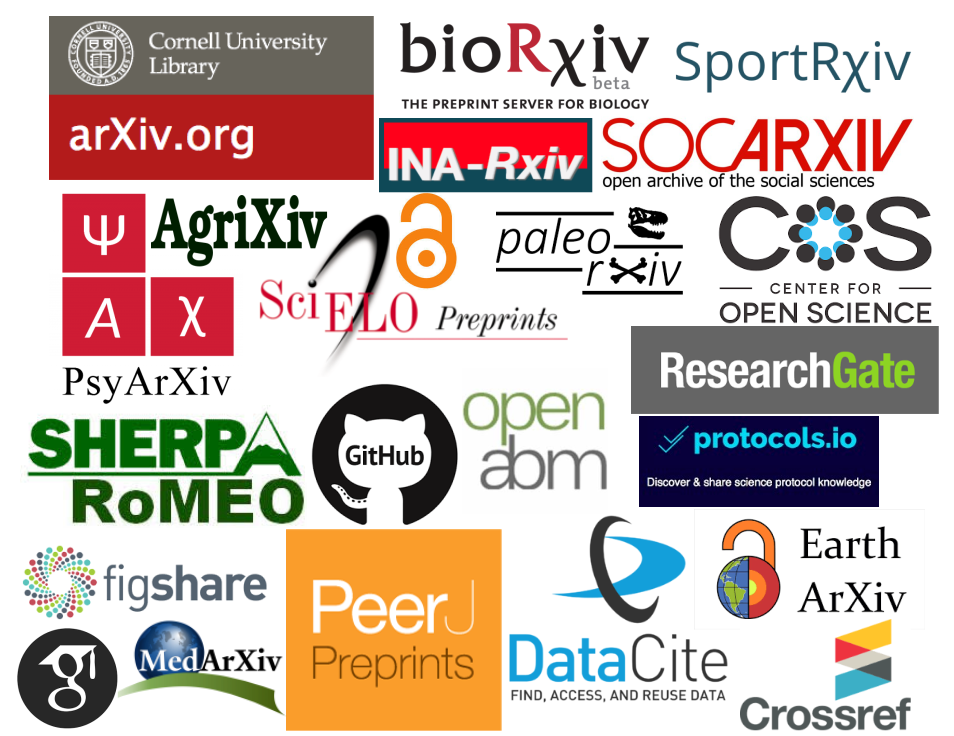
\includegraphics[width=.75\textwidth]{Arxivs}
\end{figure}
\end{frame}

\begin{frame}{Preprints como solución}
\begin{figure}
\centering
 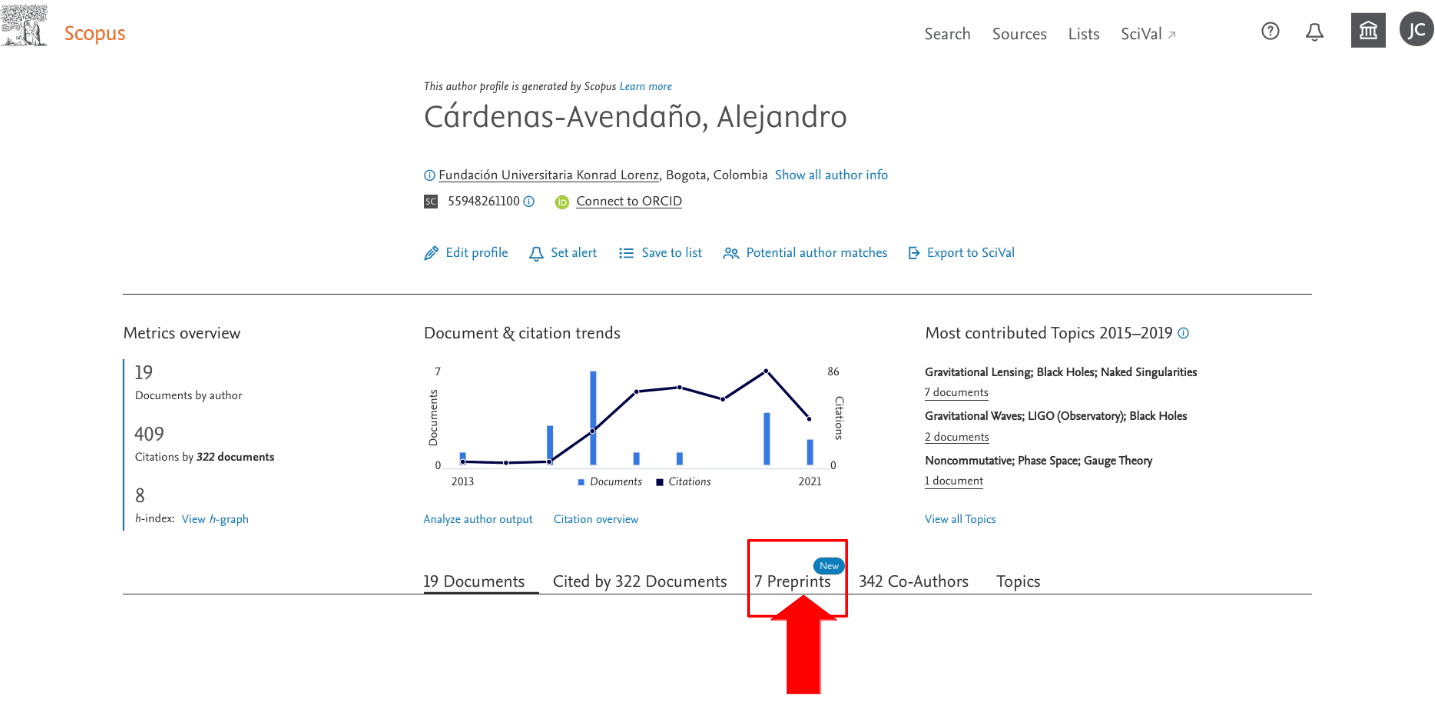
\includegraphics[width=1.1\textwidth]{PreprintScopus.png}
\end{figure}
\end{frame}

\begin{frame}{Preprints como solución}
\Large \citeauthor{Bourne2017} \citeyear{Bourne2017} proponen que:
\begin{itemize}
\vspace{0.4cm}
\item[1] Agilizan el proceso de divulgación científica.
\pause
\vspace{0.4cm}
\item[2] Deberían estar licenciados (CC-BY 4.0) para facilitar su reuso.
\pause
\vspace{0.4cm}
\item[3] Mientras los journals enfatizan validación con el peer-review, los preprints enfatizan precedencia temporal.
\vspace{0.4cm}
\pause
\item[4] Los preprints previenen el robo de ideas sin el uso de citas.
\end{itemize}
\end{frame}


\begin{frame}{Preprints como solución}
\Large
\begin{itemize}
    \item[5] Ofrecen acceso a contenido académico que de otra manera estaría invisible.
    \vspace{0.4cm}
    \pause
    \item[6] Los preprints no suponen necesariamente baja calidad.
    \pause
    \vspace{0.4cm}
    \item[7] Los preprints facilitan la rápida evaluación de resultados controversiales.
    \pause
    \vspace{0.4cm}
    \item[8] Tampoco excluyen la posibilidad de publicar en revistas indexadas y arbitradas. 
\end{itemize}
\end{frame}

\begin{frame}{Preprints como solución}
\Large
\begin{itemize}
\item[9] Facilitan la otorgación de financiamiento futuro y avance de la ciencia.
\vspace{0.4cm}
\pause
\item[10] Los preprints no significan la ``talla única'' para todo investigador (consideraciones éticas, legales, sociales).  
\end{itemize}
\end{frame}

\begin{frame}{Preprints como solución}
\begin{figure}
\centering
 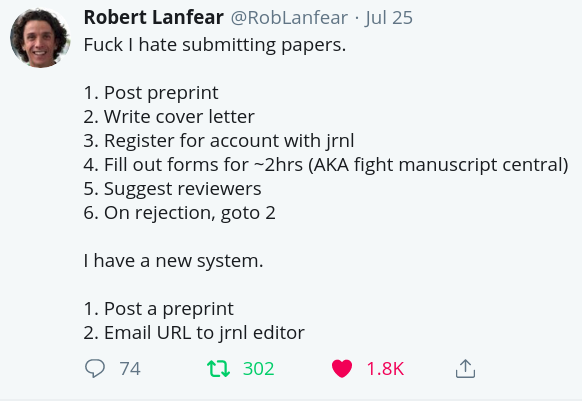
\includegraphics[width=.75\textwidth]{preprint.png}
\end{figure}
 \tiny{Tomado del perfil público de Twitter de Robert Lanfear el 25 de Julio de 2019}  
\end{frame}

\section{Preprints en la Sociedad de Psicólogos}
\begin{frame}{Preprints en la Sociedad de Psicólogos}
\Large
La Sociedad se adhiere a los principios de promoción de la apertura y transparencia documentados por la Open Science Foundation \cite{Nosek2015}. 
\begin{figure}
\centering
 
\includegraphics[width=1\textwidth]{Psyarxiv}
\end{figure}  
\url{https://psyarxiv.com/}
\end{frame}


\begin{frame}{Preprints en la Sociedad de Psicólogos}
\begin{figure}
\centering
 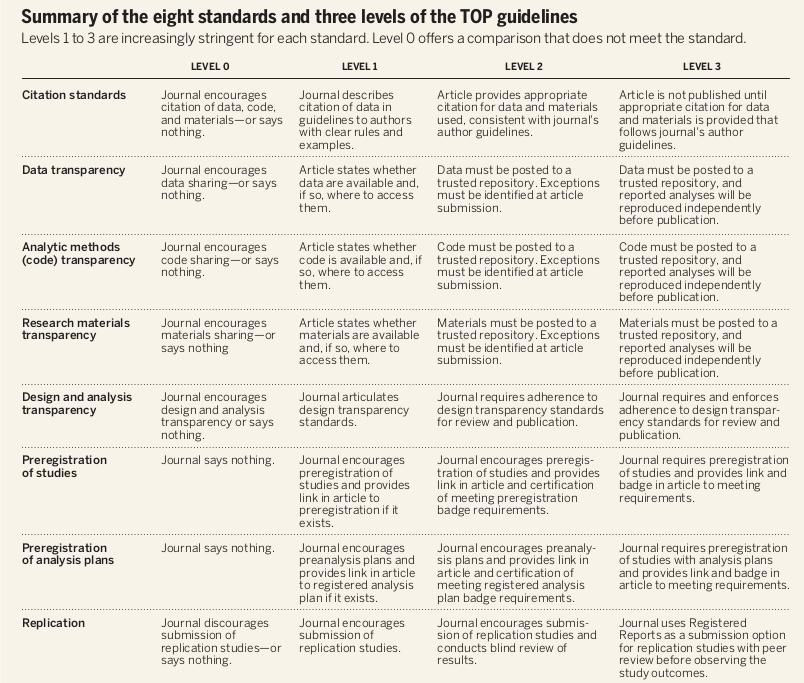
\includegraphics[width=.75\textwidth]{standards}
\end{figure}  
\end{frame}

\section{Implicaciones}
\begin{frame}{Implicaciones}
\Large
\begin{itemize}
    \item Los autores deben publicar sus datos en repositorios como Protocols.io
    \vspace{0.4cm}
    \pause
    \item Se debe hacer público los materiales (fotos, videos, encuestas) y procedimientos para la obtención y análisis de datos (incluyendo códigos computacionales, tablas y gráficos).
    \vspace{0.4cm}
    \pause
    \item Se promueve los pre-registros de análisis de datos (bases de datos no limpias, con errores en datos y sus correspondientes versiones mejoradas).
\end{itemize}    
\end{frame}

\begin{frame}{Implicaciones}
\Large
\begin{itemize}
    \item Los editores de revistas deberán decidir cuándo sumarse a esta iniciativa.
    \vspace{0.4cm}
    \pause
    \item Las revistas deben hacer explícitas las instrucciones para los autores en cuanto a los repositorios autorizados y políticas editoriales de preprints (SHERPA)
\end{itemize}    
\begin{figure}
\centering
 
\includegraphics[width=.4\textwidth]{SherpaRomeo.jpg}
\end{figure}
\end{frame}

\begin{frame}{Implicaciones}
\begin{figure}
\centering

\includegraphics[width=.75\textwidth]{nonR.png}
\end{figure}
\cite{Serra2021}
\end{frame}

\begin{frame}{Implicaciones}
\begin{figure}
\centering
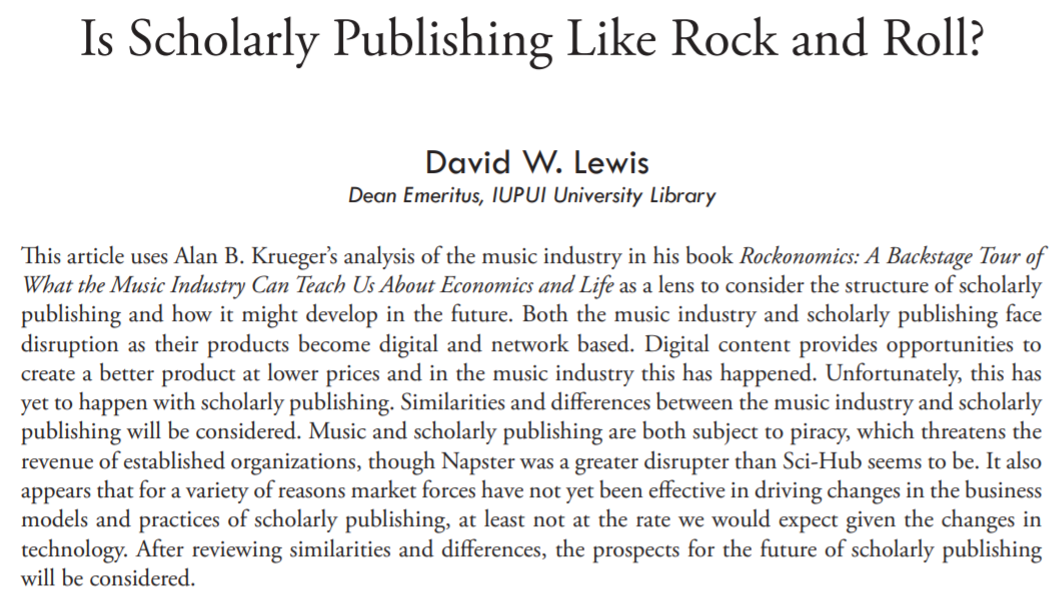
\includegraphics[width=1\textwidth]{publishing.png}
\end{figure}
\textcolor{blue}{\url{https://scholarworks.iupui.edu/handle/1805/24419}}
\end{frame}

\section{Experiencias preliminares}
\begin{frame}{Experiencias preliminares}
\begin{figure}
\centering
 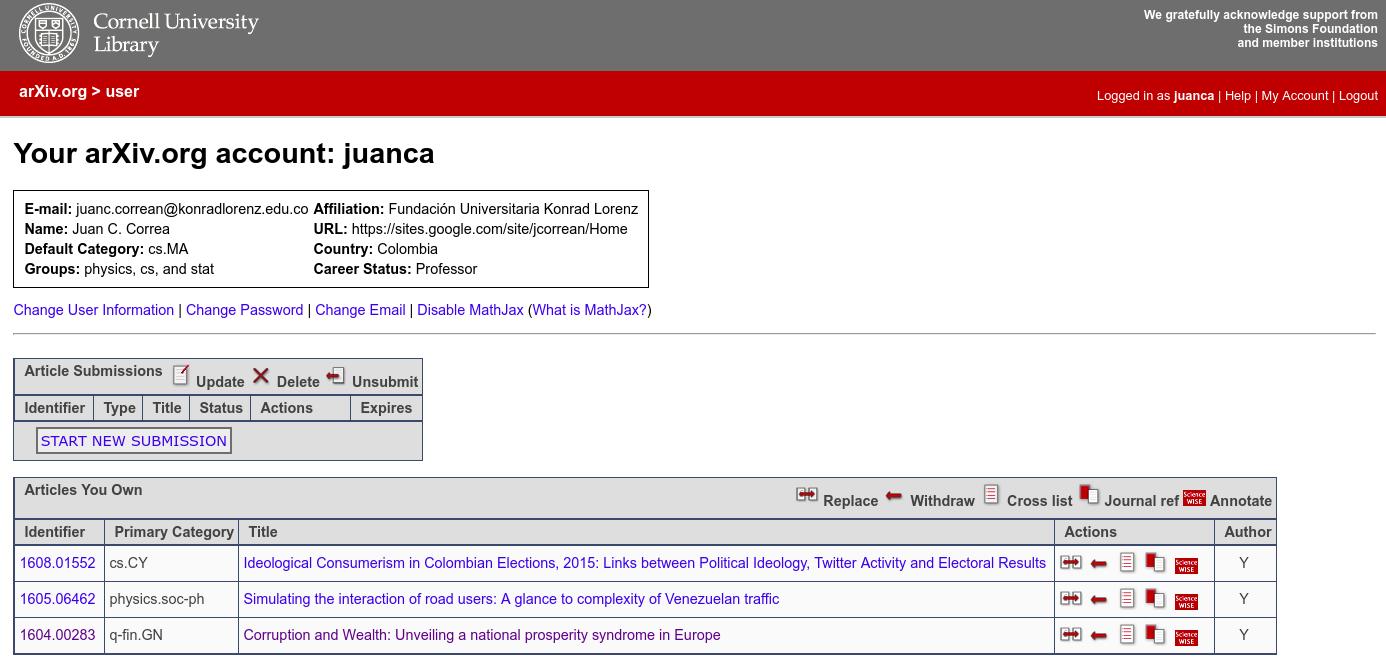
\includegraphics[width=1\textwidth]{myarxiv}
\end{figure}
\end{frame}

\begin{frame}{Experiencias preliminares}
\begin{figure}
\centering
 
\includegraphics[width=.7\textwidth]{cita2}
\end{figure}
\end{frame}


\begin{frame}{Experiencias preliminares}
\Large
\begin{figure}
\centering
 
\includegraphics[width=.9\textwidth]{ejemplo}
\end{figure}
\end{frame}


\begin{frame}{Experiencias preliminares}
\Large
\begin{figure}
\centering
 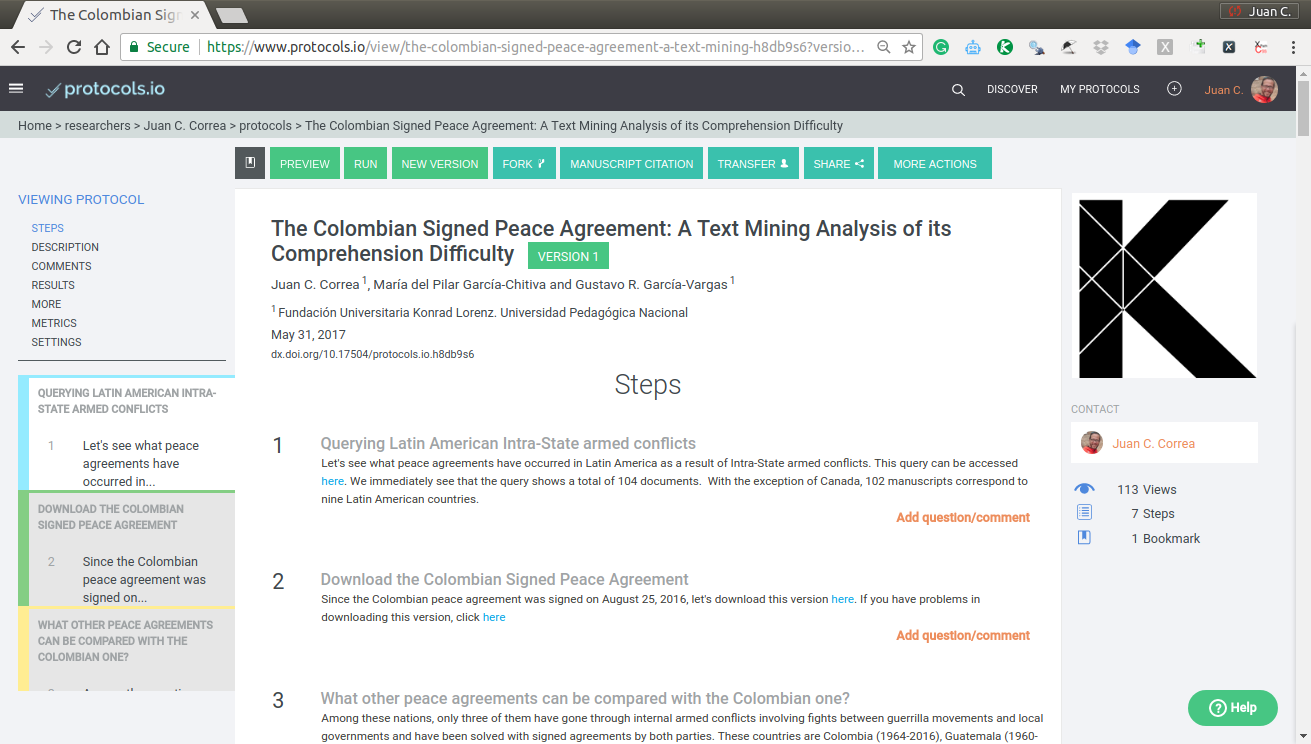
\includegraphics[width=.9\textwidth]{protocols}
\end{figure}
\end{frame}

\begin{frame}{Experiencias preliminares}
\begin{figure}
\centering

\includegraphics[width=.8\textwidth]{chupitos.png}
\end{figure}
\textcolor{blue}{\url{https://youtu.be/0LBrdPJLFIY}}
\end{frame}






\setbeamertemplate{background}{\tikz[overlay,remember picture]\node[opacity=.15]at (current page.center){\includegraphics[width=0.1cm]{LogoVice}};}
\begin{frame}
\centering
\textbf{¿Preguntas?}
\begin{figure}
\centering
 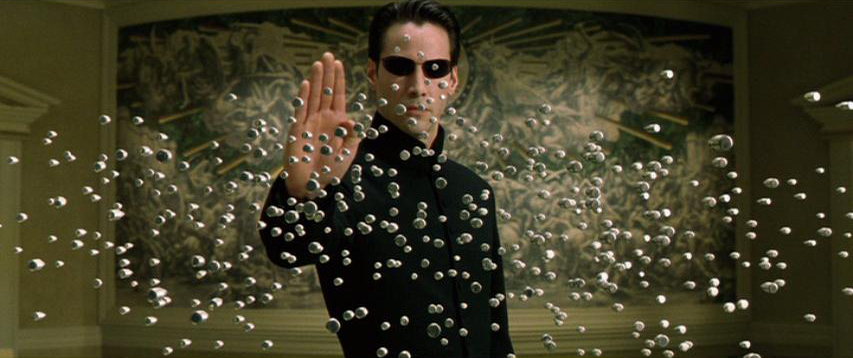
\includegraphics[width=1\textwidth]{Neo}
\end{figure}
\textbf{¡Dispara!}
\end{frame}


\setbeamertemplate{background}{\tikz[overlay,remember picture]\node[opacity=.15]at (current page.center){
\includegraphics[width=13cm]{KL}};}
%\section*{REFERENCIAS}
\begin{frame}[allowframebreaks]{Referencias}
\tiny{ 
\bibliographystyle{apacite}
\bibliography{refs}
} 
\end{frame}
\end{document}